% Tikz File 'architecture_wikibase.tex'
\documentclass{standalone}
\usepackage{tikz}
\usetikzlibrary{positioning,fit,shapes.geometric}
\begin{document}
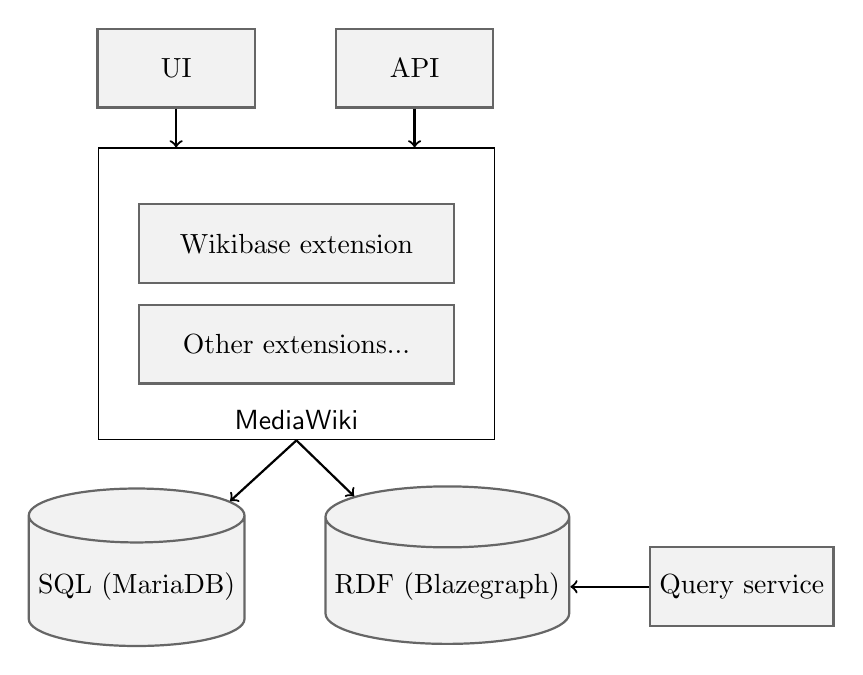
\begin{tikzpicture}[
        external/.style={rectangle, draw=black!60, fill=black!5, thick, minimum width=20mm, minimum height=10mm},
        extensions/.style={rectangle, draw=black!60, fill=black!5, thick, minimum width=40mm, minimum height=10mm},
        db/.style={cylinder, draw=black!60, fill=black!5, thick, minimum size=20mm, shape border rotate=90, aspect=0.25},
    ]
    \node[extensions] (Wikibase) {Wikibase extension};
    \node[extensions] (Others) [below=0.25cm of Wikibase] {Other extensions...};
    \node[external] (UI) [above left=1.2cm and -1.5cm of Wikibase] {UI};
    \node[external] (API) [right=of UI] {API};
    \node[db] (SQL) [below left=1.45cm and -1.1cm of Others] {SQL (MariaDB)};
    \node[db] (RDF) [right=1cm of SQL] {RDF (Blazegraph)};
    \node[external] (Query) [right=of RDF] {Query service};

    \node[fit={(Wikibase)(Others)},draw,inner xsep=5mm,inner ysep=7mm,label={[yshift=-3.7cm, font=\sffamily]MediaWiki}] (MediaWiki) {};

    \path[-to, thick] (UI.south) edge node {} (UI |- MediaWiki.north);
    \path[-to, thick] (API.south) edge node {} (API |- MediaWiki.north);
    \path[-to, thick] (MediaWiki.south) edge node {} (SQL);
    \path[-to, thick] (MediaWiki.south) edge node {} (RDF);
    \path[-to, thick] (Query.west) edge node {} (RDF.east);
\end{tikzpicture}
\end{document}